\chapter{Validazione}\label{chp:validazione}
A partire dal simulatore descritto nel capitolo \ref{chp:modello-computazionale}, di seguito sono proposte una serie di semplificazioni volte a validarlo in specifici scenari d'interesse.
\section{Blocco del flusso degli arrivi di tipo \sr{}}
Simulando il sistema privato della generazione di arrivi di tipo \sr{}, è possibile confrontare i risultati ottenuti con il modello analitico riportato in figura \ref{fig:validazione-modello-analitico-1b}.

Poiché il sistema presenta un numero $M>1$ di serventi, rispetto al modello analitico ci si aspetta un tempo d'attesa minore.
\section{Modello analitico semplificato}
\begin{figure}[ht]
\centering
\begin{subfigure}[b]{0.475\textwidth}
\centering
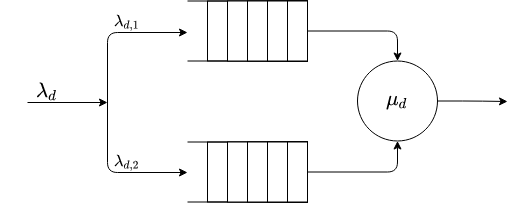
\includegraphics[width=\textwidth]{validazione-modello-analitico-1a}
\caption{Processamento di ticket \sr{}}    
\label{fig:validazione-modello-analitico-1a}
\end{subfigure}
\hfill 
\begin{subfigure}[b]{0.475\textwidth}  
\centering 
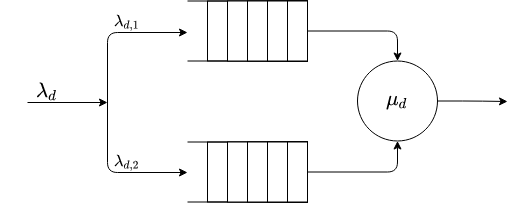
\includegraphics[width=\textwidth]{validazione-modello-analitico-1b}
\caption{Processamento degli altri ticket}    
\label{fig:validazione-modello-analitico-1b}
\end{subfigure}
\caption{Rappresentazione della semplificazione del modello}
\label{fig:validazione-modello-analitico-1}
\end{figure}

Per la validazione del modello computazionale, è stata presa in considerazione una semplificazione del caso di studio originale di seguito descritta:
\begin{itemize}
\item L'insieme degli $M-1$ serventi generali viene sostituito da un singolo servente a capacità equivalente, ovvero:
\begin{equation}
C_g = (M-1)\cdot C_{g,i}
\end{equation}
\item I tempi medi di servizio per una richiesta di tipo \uo{} o \pp{} sono equivalenti e pari a:
\begin{equation}
E[S_g] = \frac{E[S_i]}{M-1} = \frac{15}{M-1}\ min
\end{equation} 
in accordo all'equazione \ref{eqn:modello-specifiche-9} ed al bullet precedente.
\item Il $\ded{}$-esimo servente, ovvero quello dedicato, non può più processare ticket di tipo \uo{} oppure \pp{} nel caso in cui non vi siano richieste \sr{} pendenti.

Ciò implica una scissione del sistema in due partizioni tra loro isolate, come mostrato in figura \ref{fig:validazione-modello-analitico-1}.
\end{itemize}

I parametri di input del sistema così semplificato sono di seguito riportati:
\begin{itemize}
\item Le probabilità di ricadere in una determinata classe di priorità, localmente al sottosistema, sono pari a:
\begin{equation}
\begin{array}{l l}
p_{g,1} = \frac{p_{BP} \cdot p_{UO}}{p_{UO} + p_{PP}} = 0.147059, & p_{g,2} = \frac{p_{BP} \cdot p_{PP}}{p_{UO} + p_{PP}} = 0.102941, \\[1em]
p_{g,3} = \frac{(1-p_{BP}) \cdot p_{UO}}{p_{UO} + p_{PP}} = 0.441176, & p_{g,4} = \frac{(1-p_{BP}) \cdot p_{PP}}{p_{UO} + p_{PP}} = 0.308824, \\[1.5em]
p_{d,1} = \frac{p_{BP} \cdot \cancel{p_{SR}}}{\cancel{p_{SR}}} = 0.25, & p_{d,2} = \frac{(1-p_{BP}) \cdot \cancel{p_{SR}}}{\cancel{p_{SR}}} = 0.75
\end{array}
\end{equation}
dove i fattori $\frac{1}{p_{UO} + p_{PP}}$ e $\frac{1}{p_{SR}}$ sono necessari per normalizzare le probabilità originali.

I risultati ottenuti possono essere verificati con i seguenti consistency checks:
\begin{equation}
\begin{cases}
p_{g,1} + p_{g,2} + p_{g,3} + p_{g,4} = 1 & \text{\color{forestgreen}\textbf{OK} \checkmark} \\
p_{d,1} + p_{d,2}  = 1 & \text{\color{forestgreen}\textbf{OK} \checkmark}
\end{cases}
\end{equation}
\item Fissati:
\begin{equation}
\begin{array}{l l}
\lambda_g = (p_{UO} + p_{BP})\cdot \lambda = 0.207325\ req/min, & \lambda_d = p_{SR}\cdot \lambda = 0.036587\ req/min
\end{array}
\end{equation} 

I tassi medi d'arrivo sono pari a:
\begin{equation}
\begin{array}{l l}
\lambda_{g,1} = p_{g,1} \cdot \lambda_g \simeq 0.030489\ req/min, & \lambda_{g,2} = p_{g,2} \cdot \lambda_g \simeq 0.021342\ req/min, \\
\lambda_{g,3} = p_{g,3} \cdot \lambda_g \simeq 0.091467\ req/min, & \lambda_{g,4} = p_{g,4} \cdot \lambda_g \simeq 0.064027\ req/min, \\[1em]
\lambda_{d,1} = p_{d,1} \cdot \lambda_d \simeq 0.009147\ req/min, & \lambda_{d,2} = p_{d,2} \cdot \lambda_d \simeq 0.027440\ req/min \\
\end{array}
\end{equation}

I risultati ottenuti possono essere verificati con il seguente consistency check:
\begin{equation}
\begin{cases}
\lambda_{g,1} + \lambda_{g,2} + \lambda_{g,3} + \lambda_{g,4} = 0.207325 = \lambda_g & \text{\color{forestgreen}\textbf{OK} \checkmark} \\
\lambda_{d,1} + \lambda_{d,2} = 0.036587 = \lambda_d & \text{\color{forestgreen}\textbf{OK} \checkmark} \\
\lambda_g + \lambda_d = 0.243912 = \lambda & \text{\color{forestgreen}\textbf{OK} \checkmark}
\end{cases}
\end{equation}

\item I tassi di servizio medi sono pari a:
\begin{equation}
\begin{array}{l l}
\mu_g = \frac{1}{E[S_g]} = \frac{M-1}{15}\ req/min, & \mu_d = \frac{1}{E[S_d]} = 0.040196\ req/min
\end{array}
\end{equation}
dove $E[S_d] = E[S_{\ded{}, SR}]$ in accordo alla terza equazione nella \ref{eqn:modello-specifiche-12}.

\item L'occupazione media delle classi $\rho_{g,i}$ e $\rho_{d,j}$, computabile come:
\begin{equation}
\begin{array}{l l}
\rho_{g,i} = \frac{\lambda_{g,i}}{\mu_g}, & \rho_{d,j} = \frac{\lambda_{d,j}}{\mu_d}
\end{array}
\end{equation}
è pari a:
\begin{equation}
\begin{array}{l l l l}
\rho_{g,1} = \frac{0.457335}{M-1}, & \rho_{g,2} = \frac{0.320130}{M-1}, & \rho_{g,3} = \frac{1.372005}{M-1}, & \rho_{g,4} = \frac{0.960405}{M-1} \\[1.5em]
& \rho_{d,1} = 0.227560, & \rho_{d,2} = 0.682655 &
\end{array}
\end{equation}
da cui:
\begin{equation}
\label{eqn:validazione-11}
\begin{array}{l l}
\rho_g = \sum_{i=1}^4 \rho_{g,i} = \frac{3.109875}{M-1}, & \rho_d = \sum_{i=1}^2 \rho_{d,2} = 0.910215
\end{array}
\end{equation}


Dalla \ref{eqn:validazione-11} è immediato osservare che è necessario imporre $M \geq 5$ al fine di garantire la stabilità del sistema.
\end{itemize}

Il sottosistema che processa ticket di tipo \uo{} e \pp{}, riportato in figura \ref{fig:validazione-modello-analitico-1b}, è modellato con una coda $M/M/1$, per cui a partire dall'analisi teorica dei modelli a classi di priorità astratta\footnote{\label{note:validazione-1}Come nei precedenti capitoli, la priorità è inversamente proporzionale all'indice numerico della classe.}, è possibile ricavare i seguenti indici:
\begin{itemize}
\item Il \textbf{tempo d'attesa} dell'$i$-esima classe, con $i\in\lbrace 1, 2, 3, 4\rbrace$ è pari a:
\begin{equation}
E[T_{Q_{g,i}}] = \frac{\rho_g E[S_g]}{\left(1- \sum_{k=1}^{i} \rho_{g,k}\right)\left(1- \sum_{k=1}^{i-1} \rho_{g,k}\right)}
\end{equation}
da cui:
\begin{equation}
\begin{cases}
E[T_{Q_{g,1}}] = \frac{46.6481}{(M-1.457335)\cdot(M-1)}\ min \\[1.5em]
E[T_{Q_{g,2}}] = \frac{46.6481}{(M-1.777469)\cdot(M-1.457335)}\ min \\[1em]
E[T_{Q_{g,3}}] = \frac{46.6481}{(M-3.149470)\cdot(M-1.777469)}\ min \\[1em]
E[T_{Q_{g,4}}] = \frac{46.6481}{(M-4.109875)\cdot(M-3.149470)}\ min
\end{cases}
\end{equation}
\item Il \textbf{tempo d'attesa} globale è pari a:
\begin{equation}
E[T_{Q_g}]^{KP} = \frac{\rho_g E[S_g]}{1-\rho_g} = \frac{3.109875\cdot 15}{(M-1)\cdot (M-4.109875)}\ min
\end{equation}
\item Il \textbf{tempo di risposta} dell'$i$-esima classe, con $i\in\lbrace 1, 2, 3, 4\rbrace$ è pari a:
\begin{equation}
E[T_{S_{g,i}}] = E[T_{Q_{g,i}}] + E[S_g]
\end{equation}
\item Il \textbf{tempo di risposta} globale è pari a:
\begin{equation}
E[T_{S_g}]^{KP} = \frac{1}{\mu_g - \lambda_g} = \frac{15}{M-4.109875}\ min
\end{equation}
\end{itemize}

Il sistema che processa ticket di tipo \sr{}, riportato in figura \ref{fig:validazione-modello-analitico-1a}, è modellato con una coda $M/M/1$, per cui a partire dall'analisi teorica dei modelli a classi di priorità astratta\textsuperscript{\ref{note:validazione-1}}, è possibile ricavare i seguenti indici:
\begin{itemize}
\item Il \textbf{tempo d'attesa} della $j$-esima classe, con $j\in\lbrace 1, 2\rbrace$ è pari a:
\begin{equation}
E[T_{Q_{d,j}}] = \frac{\rho_d E[S_d]}{\left(1- \sum_{k=1}^{j} \rho_{d,k}\right)\left(1- \sum_{k=1}^{j-1} \rho_{d,k}\right)}
\end{equation}
da cui:
\begin{equation}
\begin{cases}
E[T_{Q_{d,1}}] = 29.315144\ min \\[1.5em]
E[T_{Q_{d,2}}] = 326.503808\ min \\[1em]
\end{cases}
\end{equation}
\item Il \textbf{tempo d'attesa} globale, per il sottosistema in figura \ref{fig:validazione-modello-analitico-1b} è pari a:
\begin{equation}
E[T_{Q_d}]^{KP} = \frac{\rho_d \cdot E[S_d]}{1-\rho_d} = 252.206642\ min
\end{equation}
\item Il \textbf{tempo di risposta} dell'$j$-esima classe, con $j\in\lbrace 1, 2\rbrace$ è pari a:
\begin{equation}
E[T_{S_{d,j}}] = E[T_{Q_{d,j}}] + E[S_d]
\end{equation}
\item Il \textbf{tempo di risposta} globale, per il sottosistema in figura \ref{fig:validazione-modello-analitico-1b} è pari a:
\begin{equation}
E[T_{S_d}]^{KP} = \frac{1}{\mu_d - \lambda_d} = 277.085065\ min
\end{equation}
\end{itemize}